\section{Spinoza and Einstein}

\begin{quotex}
The mind is its own place, and in itself can make a heaven of hell, a hell of heaven. \flright{\textsc{Satan}}

I believe in Spinoza's god, who reveals Himself in the lawful harmony of the world, not in a god who concerns himself with the fate and the doings of mankind. \flright{\textsc{Albert Einstein}}

All things excellent are as difficult as they are rare. \flright{\textsc{Benedict Spinoza}}

\end{quotex}

There is a meme going around social media based on the alleged philosophical views of Spinoza. Moreover, the claim is reinforced by reference to Einstein's approval of Spinoza. The text is ridiculous, but that hasn't stop anyone from repeating it verbatim.

Of course, they have as much chance of understanding Spinoza's \emph{Ethics} as they do of understanding Einstein's General Theory of Relativity. On the other hand, they do understand this lousy version of hippy philosophy.

\begin{wrapfigure}{rt}{.3\textwidth}
 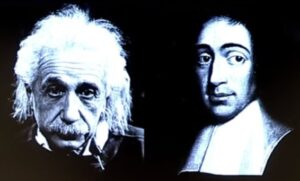
\includegraphics[scale=.5]{a20210625SpinozaandEinstein-img001.jpg} 
\end{wrapfigure}

My issue is with the meme creator. What kind of person — call him X— has such little intellectual integrity? Clearly, he has not read or understood Spinoza, yet he feels confident to fabricate quotes. Why not own up to it as his own philosophical view, rather than that of Einstein and Spinoza.

Here are some obvious bloopers:

Unlike X, Spinoza did not believe in free will. Quite the contrary, he claimed that man is driven by forces of which he is unaware and therefore keep him in bondage.

X seems to get it: ``I [i.e., God] filled you with passions, limitations, pleasures, feelings, needs, inconsistencies… free will." But he draws the wrong conclusion. As long as you are motivated by those things, you are the opposite of free.

The goal of Ethics, therefore, is self-knowledge, which does not come easily. If God does not judge you, then you need to judge yourself:

\begin{quotex}
have you ever really observed yourself consciously and uncritically and looked at yourself from this absolutely neutral angle where no self-justifying or excuses count? Or are you all the time taking yourself as yourself and thinking it is the only way to take life? \flright{\textsc{Maurice Nicoll}}

\end{quotex}
X believes in sexual excess, nowhere to be found in Spinoza. Why not, then, food excess. Why not praise gluttony or bulimia. After all, the God of X implanted the enjoyment of food as well as that of sex.

Moreover, unlike X, God does not interact with humanity, nor does he love anyone. The task is the opposite: the highest end of the person is the ``intellectual love of God."

X says: ``I am beating within you." Au contraire, mes amis, Spinoza believes in the Unity of Being. ``You" are merely a part of God, a part of the world process.

X inadvertently reveals the true source of his philosophy:

\begin{quotex}
You are absolutely free to create in your life heaven or hell. 

\end{quotex}
That is precisely Satan's philosophy as revealed by \textbf{John Milton} in \emph{Paradise Lost}.

\paragraph{Fake Philosophy}
Did you know that when Einstein gave lectures at the numerous US universities he was invited to, the recurring question that students asked him was: Do you believe in God?

And he always answered: I believe in the God of Spinoza.

The ones who hadn't read Spinoza didn't understand…

I hope this gem of history, serves you as much as it does me:

Baruch de Spinoza was a Dutch philosopher considered one of the three great rationalists of 17th-century philosophy, along with René Descartes in France, and Gottfried Leibniz in Germany.

Here's some of his wisdom:

\texttt{God would have said: Stop praying and punching yourself in the chest!}

What I want you to do is go out into the world and enjoy your life. I want you to enjoy, sing, have fun and enjoy everything I've made for you. Stop going to those dark, cold temples that you built yourself and say they are my house! My house is in the mountains, in the woods, rivers, lakes, beaches. That's where I live and there I express my love for you.

Stop blaming me for your miserable life; I never told you there was anything wrong with you or that you were a sinner, or that your sexuality was a bad thing! Sex is a gift I have given you and with which you can express your love, your ecstasy, your joy. So don't blame me for everything they made you believe.

Stop reading alleged sacred scriptures that have nothing to do with me. If you can't read me in a sunrise, in a landscape, in the look of your friends, in your son's eyes… you will find me in no book! Trust me and stop asking me. Would you tell me how to do my job?

Stop being so scared of me. I do not judge you or criticize you, nor get angry, or seek to punish you. I am pure love. Stop asking for forgiveness, there's nothing to forgive. If I made you… I filled you with passions, limitations, pleasures, feelings, needs, inconsistencies… free will. How can I blame you if you respond to something I put in you? How can I punish you for being the way you are, if I'm the one who made you? Do you think I could create a place to burn all my children who behave badly for the rest of eternity? What kind of God would do that?

Forget any kind of commandments, any kind of laws; those are wiles to manipulate you, to control you, that only create guilt in you. Respect your peers and don't do what you don't want for yourself. All I ask is that you pay attention in your life, that your consciousness is your guide.

My beloved, this life is not a test, not a step, not a rehearsal, nor a prelude to paradise. This life is the only thing that exists here and now, and it is all you need. I have set you absolutely free, no prizes or punishments, no sins or virtues… no one carries a marker, no one keeps a record.

You are absolutely free to create in your life heaven or hell.

I could tell you if there's anything after this life, but I won't… but I can give you a tip. Live as if there is nothing after… as if this is your only chance to enjoy, to love, to exist. So, if there's nothing, then you will have enjoyed the opportunity I gave you. And if there is, rest assured that I won't ask if you behaved right or wrong, I'll ask. Did you like it? Did you have fun? What did you enjoy the most? What did you learn?…

Stop believing in me; believing is assuming, guessing, imagining. I don't want you to believe in me… I want you to feel me in you when you kiss your beloved, when you tuck in your little girl, when you caress your dog, when you bathe in the sea.

Stop praising me, what kind of egomaniac God do you think I am? I'm bored being praised, I'm tired of being thanked. Feeling grateful? Prove it by taking care of yourself, your health, your relationships, the world. Express your joy!… that's the way to praise me.

Stop complicating things and repeating as a parakeet what you've been taught about me. The only thing for sure is that you are here, that you are alive, and that this world is full of wonders. What do you need more miracles for? Why so many explanations?

Look for me outside… you won't find me. Find me inside… there I am beating within you.

Spinoza.



\flrightit{Posted on 2021-06-25 by Cologero }

\begin{center}* * *\end{center}

\begin{footnotesize}\begin{sffamily}



\texttt{Michael M on 2021-06-26 at 09:46 said: }

``Spinoza believes in the Unity of Being. ``You" are merely a part of God, a part of the world process."

I have been examining this in my own experience, I found Guenon's Symbolism of the Cross helpful and timely.

``In each being envisaged in particular, this spark of the intelligible Light constitutes, if one may so put it, a fragmentary unity (an expression inaccurate if taken literally, for unity is really indivisible and without parts)."

My understanding of what Guenon goes on to say is that the Man, in his proper term, will then reflect the properties of Being given that he is of Being, though from the view of manifestation it can appear that Being is ``within" him so to speak. (Micro/Macrocosm being displayed)

This meme creator says consciousness needs to be a guide and as much as I want to give X the benefit of the doubt, he seems to bank on the error, well put by Barfield, that everyone has and has had the same consciousness throughout history and is somehow on equal footing to talk about God, let only some life ``philosophy". How is it that the modern mind, understanding how infinitely small it is even in just a material sense, can find itself capable of trying to juxtapose what God would ``say" in the form of a dead man's name?

30 blows on the head would be too compassionate for this one.


\hfill

\texttt{Sylvan Savant on 2021-07-14 at 00:22 said: }

I quite wanted to retch while reading that alleged ``Spinoza" shitpost. If the quote cited here is the best he can come up with, it's no wonder the devil has been overtaken by Mammon and Elon Musk.

I mean it's such a low hanging fruit that it can only appeal to the Gen-X American consumer mentality, which the adversary realized had run its course. The great temptation of the future will not come from this hedonistic sappy nonsense, but from the human desire to see truth and justice raised to the absolute in the social environment. The subtle whispers will that one be making into the ears of future Savonarolas and Hitlers, the seekers of ruin in the name of justice.


\hfill

\texttt{Dimitri on 2023-03-26 at 19:10 said: }

Would you recommend reading Spinoza or could he be skipped?


\hfill

\texttt{Cologero on 2023-03-28 at 19:05 said: }

Skip him, unless you have a lot of free time.


\end{sffamily}\end{footnotesize}
